\chapter{FREEFLOW}
\label{ff}
The Freeflow project aims to bridge the gap between high level network
programming languages and low level networking hardware by defining an ideal
execution environment for network applications. Evaluating the benefits and
deficits with respect to flexibility and performance provides a more accurate
level of translation or abstraction to use. In Figure \ref{ff_arch}
the Freeflow system architecture is illustrated.

\begin{figure}[h]
\centering
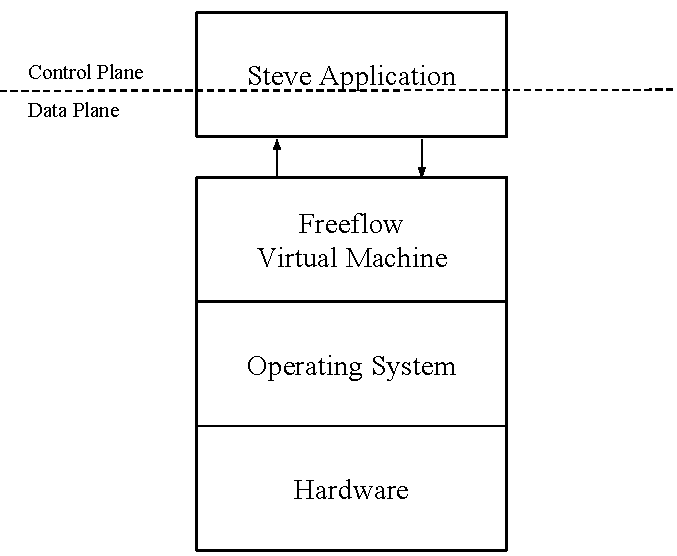
\includegraphics[scale=0.5]{ff_arch}
\caption{FFVM provides computational and memory resources to applications.}
\label{ff_arch}
\end{figure}

This chapter elaborates on the Freeflow programmable virtual switch
implementation details. The first few sections describe how applications are
hosted and how packet data is represented and manipulated. In the remainder of
the chapter, the virtual machine and its components are discussed. These include
object models for ports and tables, dynamic instruction execution, as well as
the memory and threading models supported.

% \section{Control Plane}
% \label{ff:cp}
% The control plane acts as the brain in a network switch, and is responsible for
% the configuration and management of the underlying data plane. In an FFVM
% virtual switch, control logic is provided by a hosted network application that
% is dynamically loaded. The application
%
% In the control plane, the system configuration establishes the resources
% that must be provided to support application execution. During execution,
% events raised from the data plane are caught and processed by application
% defined event handlers in the controller.
%
% \section{Data Plane}
% \label{ff:dp}
% A data plane executes the forwarding behavior for traffic flows using a variety
% of hardware, and sometimes software, constructs available in a given system. The
% FFVM data plane provides the necessary resources to host compiled network
% applications.

\section{Application Hosting}
\label{ff:app}
Freeflow applications provide the logic for the control and data planes in the
switch. This is a departure from common SDN solutions, where the two planes are
treated as separate entities and typically distributed across many devices.
The reason for blurring the line between the two parts is to reduce the overhead
penalty that is incurred in the former model. By allowing the application to
straddle the line between the control and data planes, the logic it provides is
able to be pushed into the appropriate hardware and executed efficiently.

\begin{figure}[h]
\centering
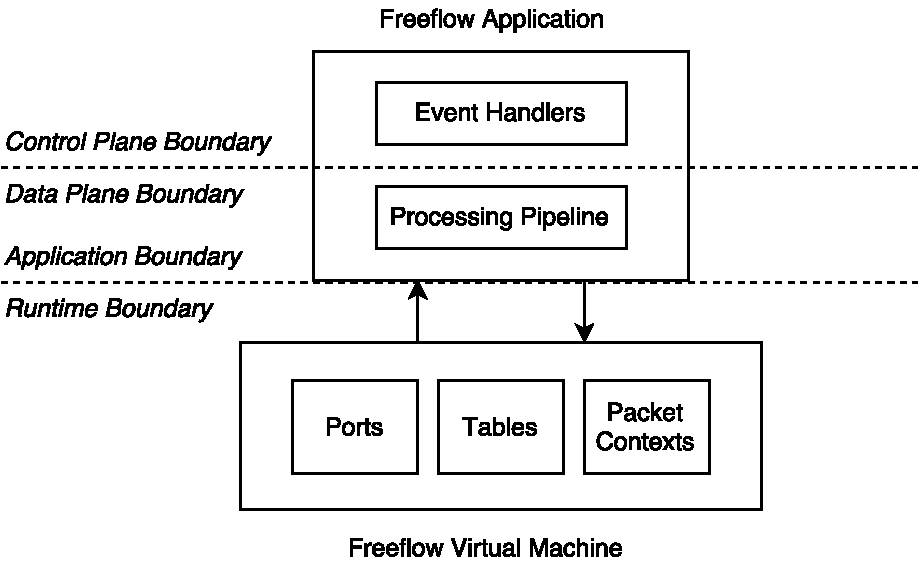
\includegraphics[scale=0.5]{application}
\caption{Freeflow application logic spans across multiple boundaries.}
\label{app}
\end{figure}

Networking applications operate on packets, utilizing information found inside
of nested protocol headers to determine the appropriate action to take. In
Freeflow, applications and the virtual machine operate on packet contexts
that store contextual information about a packet in the system. Applications
use these contexts to process packets in a series of stages that extract
protocol information and apply rule matching logic to them. A typical
application pipeline is illustrated in Figure \ref{app_pipeline}.

\begin{figure}[h]
\centering
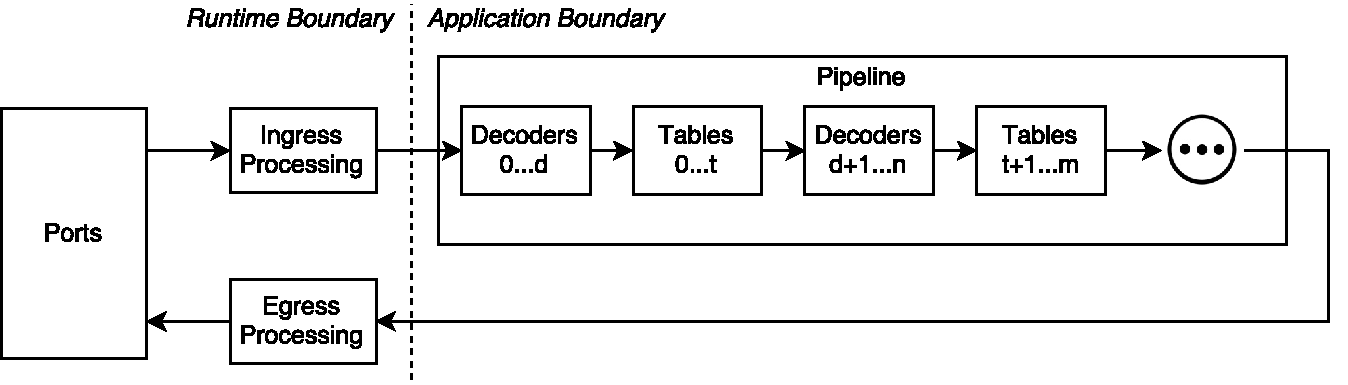
\includegraphics[scale=0.5]{app_pipeline}
\caption{Freeflow applications define a list of decoders and tables.}
\label{app_pipeline}
\end{figure}

Freeflow applications are loaded dynamically through application binary
files, compiled to native shared object libraries. Currently only one instance
of an application binary can be loaded into a FFVM process space. The FFVM
calls functions, exported as symbols from the binary, to manipulate the state
of the application. Freeflow application state is defined as:

\begin{itemize}
  \item \texttt{init} - All exported symbol handles have been resolved.
  \item \texttt{ready} - The application is loaded and able to start.
  \item \texttt{running} - The application is being executed.
  \item \texttt{stopped} - The application is halted.
\end{itemize}

The functions that control the application life cycle all require a handle
to the host data plane in order to provide dynamic allocation of resources.
These functions are:

\begin{lstlisting}
    ff_load(dp);
    ff_unload(dp);
\end{lstlisting}

The \texttt{ff\_load} function initializes global data plane resources required
by the application, such as tables. When successful the application state is
set to ``ready'', or is left in an ``init'' state when errors occur. During
FFVM tear down, a call to \texttt{ff\_unload} will release the allocated
resources if the application is not in a ``running'' state.

\begin{lstlisting}
    ff_start(dp);
    ff_stop(dp);
\end{lstlisting}

Applications ``learn'' about state and configuration changes to the data plane
they are hosted in through events. The \texttt{ff\_start} function sets the
application state to ``running'', starting packet processing and allowing events
to be handled. A call to start is only valid when the state of the application
is ``ready'' or ``stopped''. The \texttt{ff\_stop} function halts packet
processing, disables event handlers, and sets the state to ``stopped''.

\begin{lstlisting}
    ff_process(cxt);
\end{lstlisting}

The application defines the forwarding behavior for a data plane by providing
a packet processing pipeline. After a packet is received and exits ingress
processing, the FFVM calls the process function on a packet context. In order
to forward packets, the application must provide the definition of a packet
processing pipeline for the FFVM to execute.

\section{Packet Context}
\label{vm:packet-context}
Network packets are arranged as nested protocol headers, which contain fields
that describe the structure and contents of a particular layer. Since the
Freeflow data plane has no knowledge of any protocol structures (i.e. it is
protocol independent), it operates on contextual information extracted by
applications and stored in a \emph{context} object. The meta data contained
in a context allows the data plane to provide robust network functionality
and execute a variety of network applications.

\subsection{Packets}
In networking, packets represent raw data that have been transmitted over some
media with protocol headers for each layer contained in the packet. Each header
gives information about the structure and state of the current protocol being
processed. Figure \ref{ipv4_eth_frame} shows an example Ethernet frame
(packet) containing an IP (v4) header.

\begin{figure}[h]
\centering
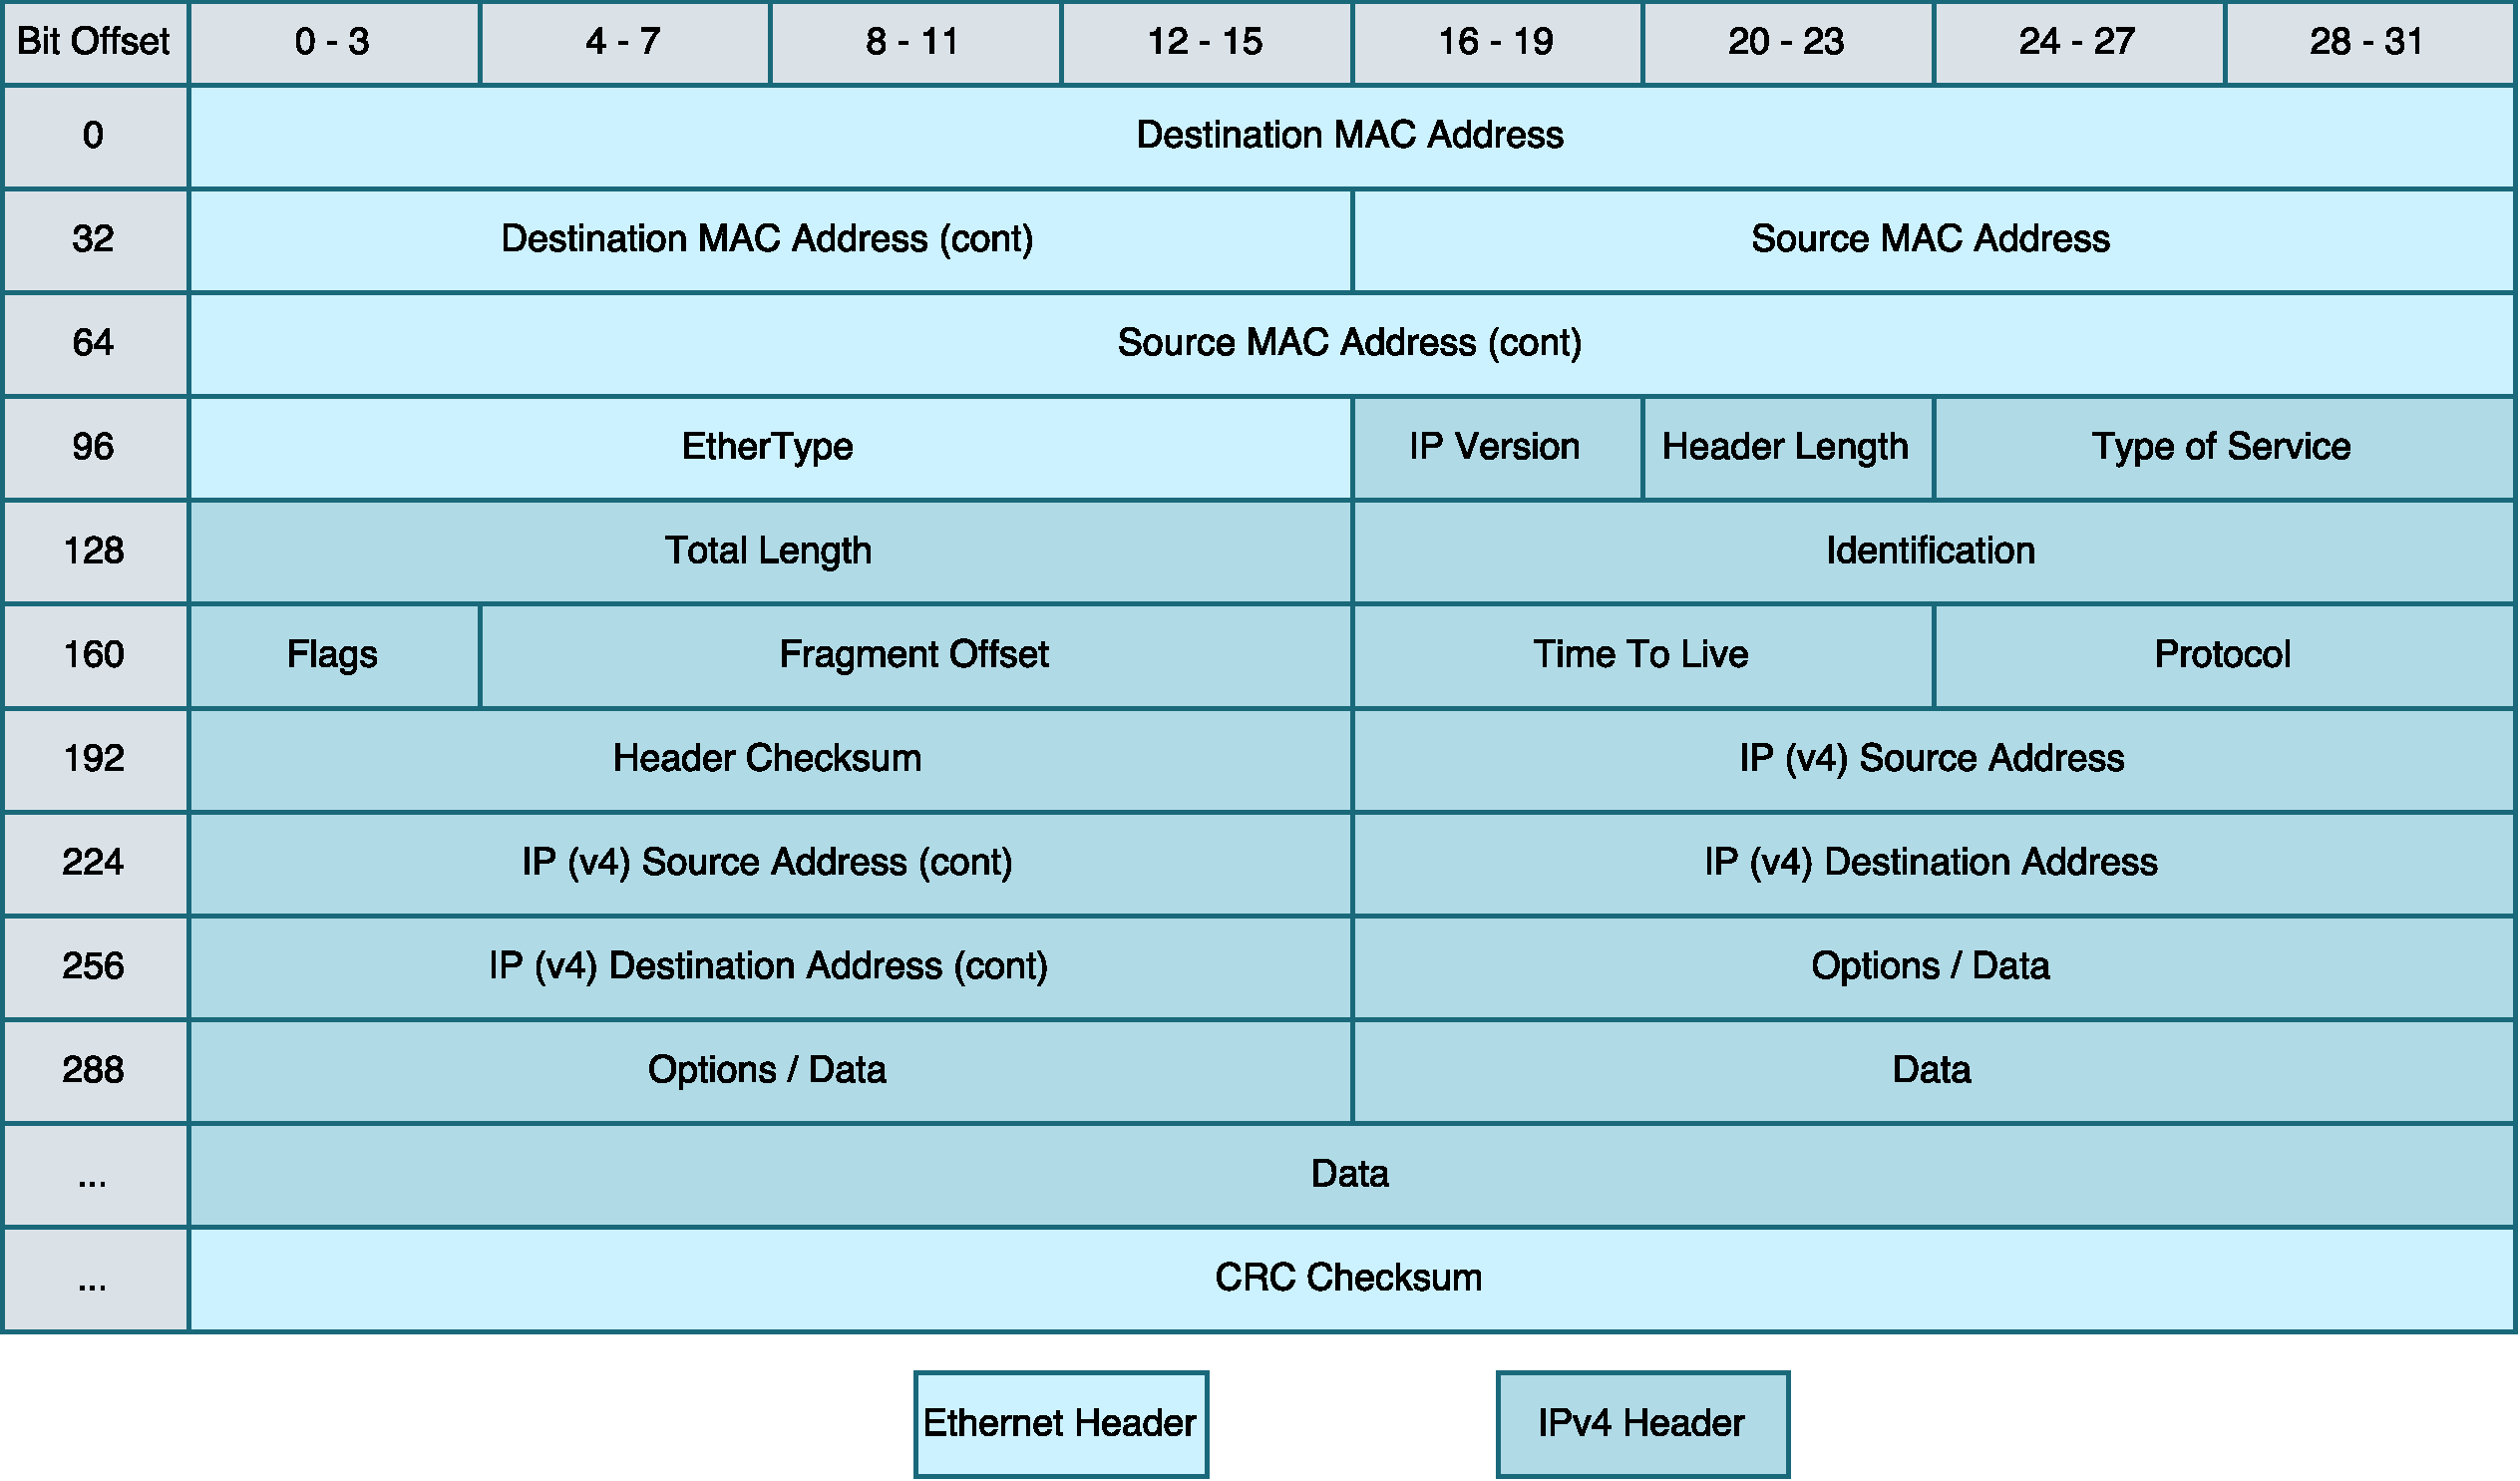
\includegraphics[scale=0.33]{ipv4_eth_frame}
\caption{An IPv4 Ethernet frame.}
\label{ipv4_eth_frame}
\end{figure}

The layout for each protocol is far from uniform, and fields within headers do
not always align to the traditional byte-aligned boundaries (e.g. Ethernet
MAC addresses which have a width of 48 bits). Storing these values in memory
results in wasted space, as larger data structures would need to be utilized.
Structure packing pragmas and bit width specifiers can be used to overlap
memory regions when the desired bit width is less than the standard width for
that type (e.g. \texttt{std::int\_64:48;}). However storing a copy of the
packet data would result in coherency issues, negatively impacting
performance. Instead the fields within headers are stored in a \emph{binding
environment}, discussed in the following section.

\subsection{Context}
The packet \emph{context} provides contextual information about an associated
packet in the system. A context is where applications store input, control, and
decoder information, as well as application meta data. This is also where they
build action lists.
Input information consists of data about the packets arrival into the system,
such as the input logical and physical ports. The control information maintains
the control flow of a context as it traverses processing pipelines.

\begin{lstlisting}
struct Decode_info {
  uint16_t    pos;     // Packet decoding offset
  Environment headers; // Saved packet header locations
  Environment fields;  // Saved packet fields locations
};

struct Context {
  Ingress_info input;
  Control_info ctrl;
  Decode_info  decode;
  Packet       packet;   // A handle to packet memory
  Metadata     metadata; // Application-defined metadata
  Action_list  actions;  // A sequence of instructions
};
\end{lstlisting}

As application packet decoders execute, they store the position, or offset, and
length of the desired fields as pairs in a binding environment, referred to as
the decode information. This environment notes the offset of a field within the
current protocol header, as well as the offset for each protocol header within
the packet buffer. Utilizing this heavy weight approach to referencing protocol
field information enforces a more precise data extraction plan and eliminates
coherency issues. Figure \ref{context_binding} shows the resulting binding
environment created after decoding the Ethernet source and destination fields,
as well as the IPv4 protocol and destination fields.

\begin{figure}[h!]
\centering
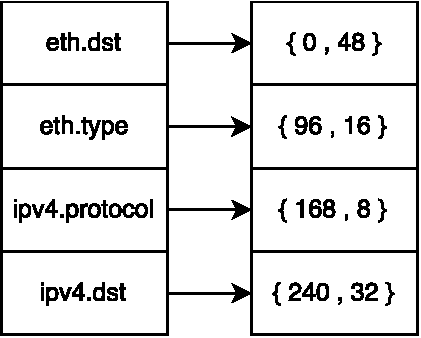
\includegraphics[scale=0.9]{context_concrete}
\caption{An example binding environment for an IPv4 Ethernet frame.}
\label{context_binding}
\end{figure}

The raw packet data is accessed through a handle held by the context. Depending
on the capabilities of the port that received the packet, this handle may point
to a Freeflow packet buffer or dedicated port memory. Meta data provides
``scratch'' space for applications to store additional information during
pipeline processing. The action list is composed of instructions that are to
be applied to a packet after exiting an application pipeline but before egress
processing. These instructions are used to modify fields within a packet, and
are explained further in Section \ref{vm:insn}.

\section{Virtual Machine}
\label{vm}
The Freeflow Virtual Machine is composed of modular parts that a programmer can
assemble into a virtual switch. This flexibility allows for the instantiation
of numerous switches with varying features and capabilities. In general,
switches require control and data planes as well as compiled network
applications to drive each component. A FFVM virtual switch can be assembled
by creating a data plane instance, in which port resources are added and an
application is loaded. User space drivers provision the machine with these
components and execute compiled applications. An example driver is shown in the
following listing.

\begin{lstlisting}
// Create a data plane instance named `dp1'.
ff::dataplane dp = ``dp1";

// Add virtual (internal) ports and two TCP sockets.
dp.add_virtual_ports();
ff::Port* port1 = new ff::Port_tcp(1);
ff::Port* port2 = new ff::Port_tcp(2);
dp.add_port(port1);
dp.add_port(port2);

// Load a sample application named `sample.app'.
dp.load_application(``sample.app");

// Set data plane configuration to `up',
// starting execution.
dp.up();
\end{lstlisting}

The driver makes a virtual switch with a single data plane, named ``dp1'', that
contains the predefined virtual ports and two TCP ports, with i.d.s 1 and 2
respectively. After allocating port resources, an application named
``sample.app'' is loaded, allowing the system to perform table configuration
and import the pipeline processing symbols. Figure \ref{ff_system} illustrates
the orchestration of the components utilized in the example driver listing.

\begin{figure}[h]
\centering
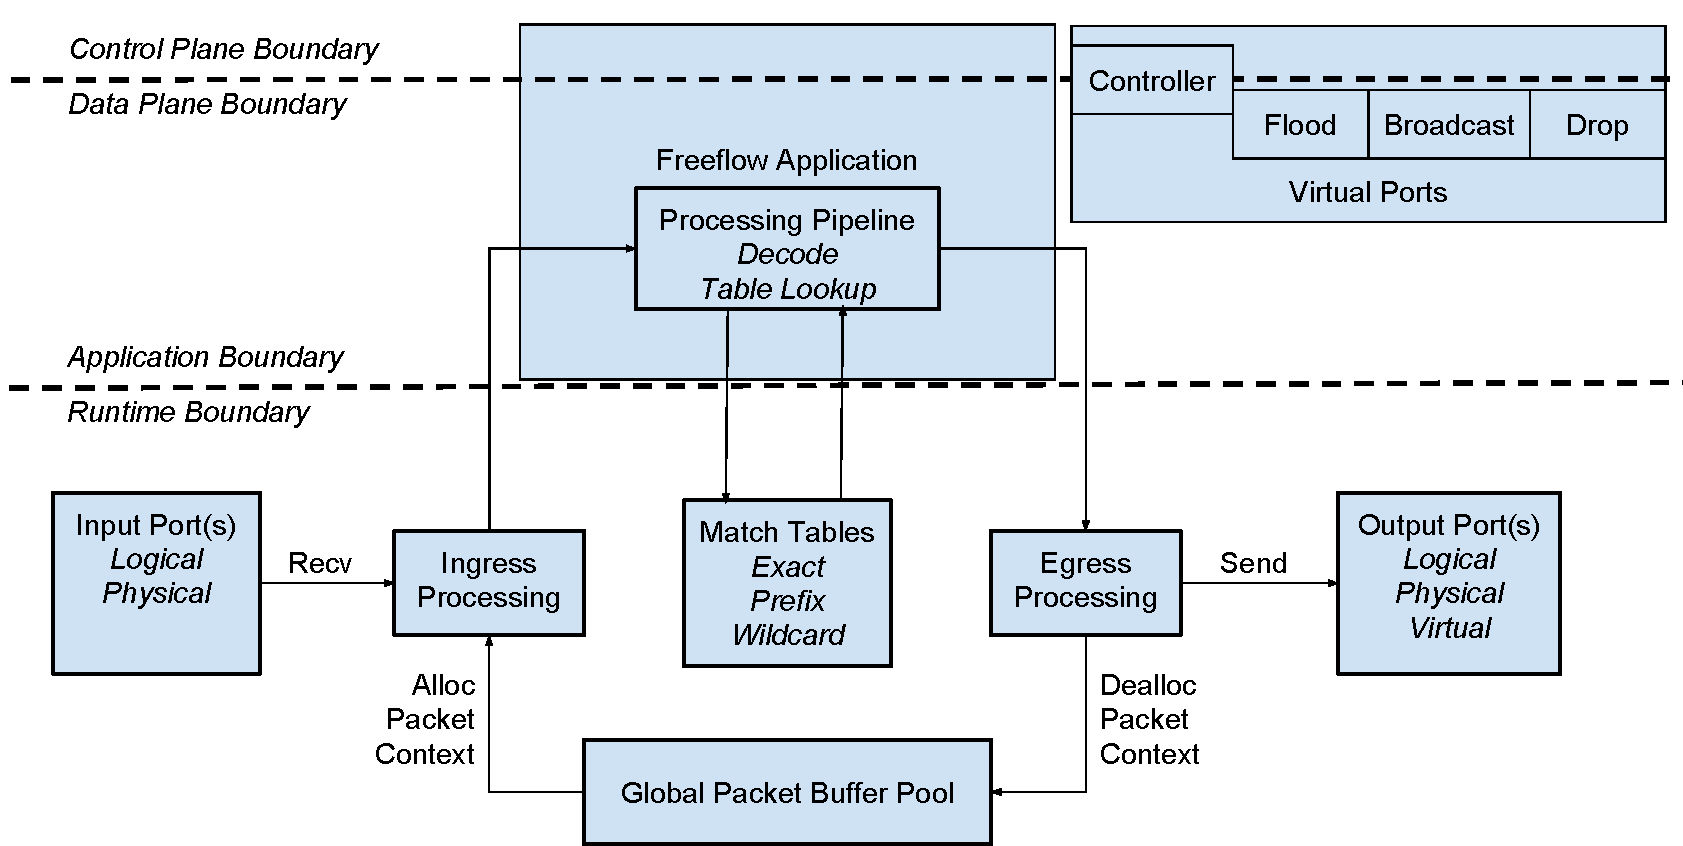
\includegraphics[scale=0.53]{ff_system}
\caption{The Freeflow virtual switch architecture.}
\label{ff_system}
\end{figure}

\section{Ports}
\label{vm:port}
Ports act as the main source of I/O for network applications. They provide the
means to receive and send packets that are entering and leaving the system. As
an abstract type, the port interface is fairly simple. Any derived port object
needs only implement the following four functions:

\begin{itemize}
\item Send - Transmit packet data.
\item Receive - Retrieve packet data.
\item Up - Puts the port into a usable state, data can be sent and received.
\item Down - Disables port functionality.
\end{itemize}

Port objects can be classified as being physical, logical, or virtual. A
physical port represents a hardware networking interface, e.g. Ethernet cards.
Logical ports represent software networking constructs that utilize file
descriptors to act as an endpoint for communication. An illustration of the port
object UML can be found in Figure \ref{port_uml}. Virtual ports are derived
from logical ports, and provide specialized functionality for the system. To
further classify the port type, they can be either seen as an \emph{input}
port, where data from an external source can be ingressed into the system, or an
\emph{output} port, which sends data to other external or internal devices.
Currently input ports can be either logical or physical, whereas output ports
can be any port type (i.e. logical, physical, virtual).

\begin{figure}[h]
\centering
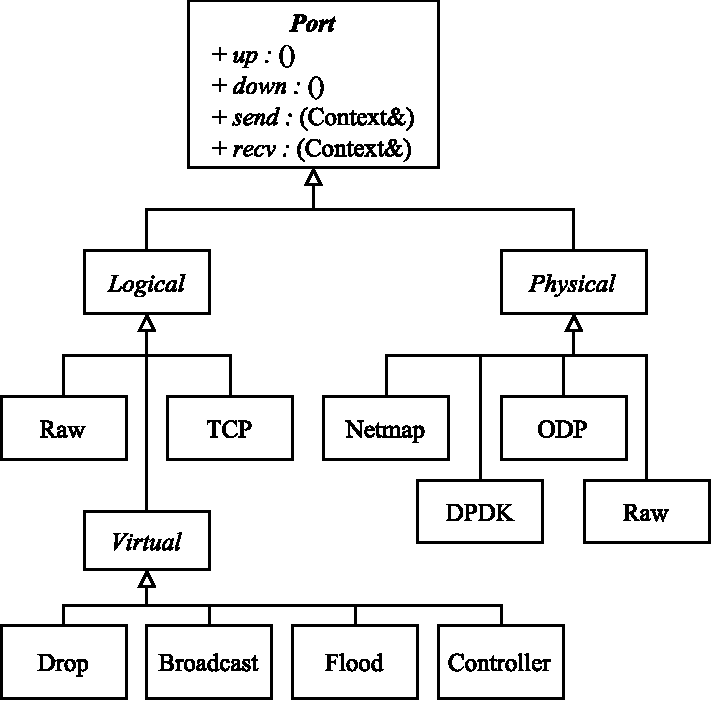
\includegraphics[scale=0.85]{ff_port_uml}
\caption{Freeflow port UML diagram.}
\label{port_uml}
\end{figure}

When packets are received by a port object, the memory that holds the raw
packet data and the context are allocated during the \emph{ingress} phase. The
underlying data store for the packet and context are owned and managed by the
port itself. Memory can be allocated from the ports internal resources (i.e.
memory mapped from a physical device address space) if present, or by the FFVM's
global buffer pool. This gives a greater amount of flexibility in that the
packet and context can exist in same memory region, potentially improving
locality. As packets leave the system during the \emph{egress} phase, this
memory is released back to the appropriate devices. Details about memory
management can be found in Section \ref{vm:memory}.

After initializing a context with a new packet, the port passes the context to
the application pipeline for processing. When the context exits the application
pipeline, the resulting action list is applied to the packet. Finally the
context enters the egress stage where the packet is forwarded to the designated
\emph{output port} set in the context, or dropped.

% The freeflow port impl lies somewhere on the spectrum...

\section{Tables}
\label{vm:tables}
In network switches, tables are used to match properties of packets
with user-defined forwarding behaviors. They can be defined using a variety of
data structures and algorithms that implement them, but generally are categorized
as \emph{exact}, \emph{prefix}, or \emph{wild card}. All three table types are
currently implemented by the FFVM, though support for prefix and wild card is
incomplete.

Each entry in a flow table contains a \emph{key} that is compared to a
certain field within the packet. Key types vary between match table types. For an
exact match table the keys are integers of a set width, defined by the
application. These keys are used to aggregate traffic containing similar
characteristics into flows. Flows can be viewed as programs, or functions,
that get executed when a packet matches their key. Each flow defines a
set of operations, or instructions, that are applied to packets. Table
\ref{flow_table} depicts a simple flow table that creates a virtual ``wire''
between two ports, where traffic received by one port is sent out the other.

\begin{table}[h]
  \centering
  \begin{tabular}{||c | c||}
   \hline
   Input Port & Flow Instruction \\ [0.5ex]
   \hline\hline
   1 & output(2); \\
   \hline
   2 & output(1); \\
   \hline
   miss & drop; \\ [1ex]
   \hline
 \end{tabular}
 \caption{A flow table that maps input ports to output ports.}
 \label{flow_table}
\end{table}

% The freeflow table impl lies somewhere on the spectrum...

\section{Instructions}
\label{vm:insn}
The FFVM hosts network applications that are dynamically loaded and executed
at run time. To avoid using an interpreter, applications must be compiled
to native shared objects. By translating the high level language down to the
target machine code, the execution of instructions provided in the binaries is
more efficient. These instructions are encapsulated in functions that can be
executed on a variety of computational devices. This allows the FFVM to take
advantage of hardware accelerators tuned for network processing.

% Freeflow insn execution lies somewhere on the spectrum...

\section{Memory}
\label{vm:memory}
Memory for raw packet data and contexts is allocated by port objects during the
ingress processing phase. The FFVM is optimized to allow for zero-copy packet
processing, where raw packet data resides in a physical device's dedicated
memory. In certain cases device packet buffers contain extra memory for user
data, which can store the context object to improve locality. Another
benefit of storing the packet and context in the same region of memory is that
the two entities can grow dynamically; the context grows as actions are appended
to it's action list and the packet grows when new protocol headers are pushed
onto a header binding environment. When a port object does not possess the
capability to provide persistent packet memory, a global packet context buffer
can be allocated by the system. Figure \ref{mem_model} illustrates the two
memory models currently supported by the FFVM.

\begin{figure}[h]
  \centering
  \begin{subfigure}[b]{0.48\textwidth}
    \centering
    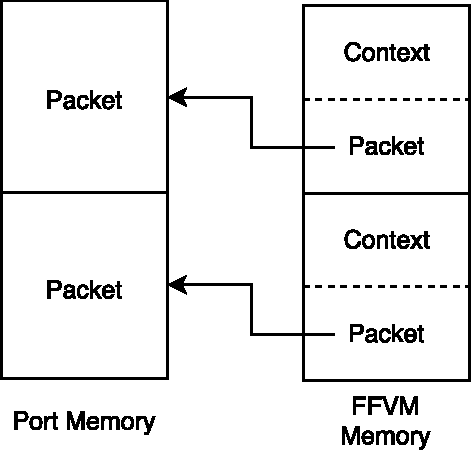
\includegraphics[scale=0.9]{mem_fig_a}
    \caption{Freeflow allocates context memory that references packet data
    in port memory.}
  \end{subfigure}
  \hfill
  \begin{subfigure}[b]{0.48\textwidth}
    \centering
    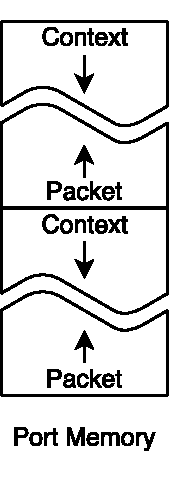
\includegraphics[scale=0.9]{mem_fig_b}
    \caption{Port memory can accommodate dynamically sized packet and context
    objects.}
  \end{subfigure}
  \caption{Freeflow packet context memory models.}
  \label{mem_model}
\end{figure}

A global buffer consists of a packet buffer, a context, and a non-zero
i.d. Packet buffers are pre-allocated 2048 byte regions that can easily
accommodate IEEE 802.3 Ethernet frames that have a maximum size of 1523 bytes.
The packet buffers are over sized to allow for the insertion of new protocol
headers that may result during or after pipeline processing. Contexts residing
in a global buffer contain a reference to the packet buffer, which by default
points to a FFVM packet buffer. The i.d. gives the offset into the global buffer
pool, and allows ports to return the i.d. back to the pool's free list. FFVM's
free list is implemented as a min-heap, providing the next available packet
buffer that can be allocated. During creation, and upon de-allocation, a packet
context buffer is set to a null state; each field in the context is default
initialized and the packet size is set to 0. In this state, referencing a
context or the packet buffer it is associated with is undefined.

% The freeflow memory model lies somewhere on the spectrum...

\section{Threading}
\label{vm:threading}
The FFVM supports multiple threading architectures to maximize execution
resource utilization. Behavior for FFVM components, such as port objects and
application pipelines, can be defined as free functions in a driver and
executed in its own thread. Threads contribute to the modular nature of the
FFVM and can be treated as building blocks to produce different execution
models. FFVM provides a simple threading interface built on the POSIX thread
library (pthread) \cite{pthread}, that executes a preallocated work routine
and passes the thread i.d. as the argument. Synchronization mechanisms and
configuration settings, or attributes, are optionally provided. The following
listing shows how a FFVM thread can be constructed with an initial i.d. and work
routine, and also re-assigned while the thread is not in a ``running'' state.

\begin{lstlisting}
void* port_work(void* arg){
  // ...
}

void* port_work2(void* arg){
  // ...
}

int main(int argc, char** argv){
  ff::Thread thread = { 1, port_work };
  thread.run();
  // ...
  thread.halt();
  thread.assign(2, port_work2);
  thread.run()
  // ...
  thread.halt();
  return 0;
}
\end{lstlisting}

In addition to the threading interface, the FFVM also provides shared data
structures such as queues and object pools. Concurrent queue implementations
exist for locked and lock-free access, allowing for more flexibility in the
threading architecture being modeled. Object pools allocate reusable global
resources that can also be shared across thread boundaries.

\section{ABI}
\label{vm:abi}
The FFVM application binary interface exposes a set of symbols and calling
conventions that can be utilized by applications at run time. These ``system
calls'' allow hosted applications to request system resources. In this section
the more pertinent functions are discussed.

\begin{lstlisting}
    ff_create_table(dp, width, n, type);
    ff_delete_table(dp, tbl);
\end{lstlisting}

A call to the \texttt{ff\_create\_table} function returns a newly allocated
flow table in the given data plane instance \emph{dp} with an application
defined key \emph{width} in bytes, an initial size of \emph{n} entries, and
matching table \emph{type}. The \texttt{ff\_delete\_table} call releases the
resources allocated in the given table \emph{tbl}.

\begin{lstlisting}
    ff_lookup_flow(tbl, k);
    ff_insert_flow(tbl, k, f);
    ff_remove_flow(tbl, k);
\end{lstlisting}

Flow entry matching is executed with a call to \texttt{ff\_lookup\_flow} which
searches for a key \emph{k} in a flow table \emph{tbl}. Table modifications can
be made using \texttt{ff\_insert\_flow} to add a new key \emph{k} with the
flow \emph{f} to table \emph{tbl}, and \texttt{ff\_remove\_flow} to remove the
key \emph{k} from the table \emph{tbl}. If the key already exists when the call
to insert is made, the associated flow object is updated, whereas a call to
remove a non-existent key from a table has no effect.

\begin{lstlisting}
    ff_output(cxt, p);
    ff_drop(cxt);
\end{lstlisting}

The \texttt{ff\_output} function sets the \emph{output\_port} field in a context
\emph{cxt} to the id of the given port \emph{p}. A call to the \texttt{ff\_drop}
function effectively sets the \emph{output\_port} field in the context \emph{cxt}
to the data plane drop port id, but terminates the further processing in the
pipeline stage it was invoked from.

\section{Conclusion}
\label{ff:concl}
Freeflow embodies the contributions made in this thesis. All of the components
developed make Freeflow a framework for creating virtual programmable switches.
The modular approach allows the VM to be re-configurable at run time where it
can dynamically change shape with respect to resources, ports and memory, and
functionality from real time updates to forwarding rules. We choose this model
in order to create and evaluate different switch architectures and threading
models. In order to work towards an ideal execution environment for hosted
network applications, Freeflow gives the ability to test and narrow the set of
requirements that are necessary to achieve this goal.
